% BEGIN TEMPLATE
\documentclass{article}
\usepackage{graphicx}
\usepackage{hyperref} 
\usepackage{xcolor}
\usepackage{nameref}
\usepackage{listings}
\usepackage{subcaption}
\usepackage{float}
\usepackage[title]{appendix}
\graphicspath{ {../../images/} }
% CHANGE THESE
\newcommand{\courseListing}{CSCI 8110-001}
\newcommand{\courseName}{Advanced Machine Learning Applications}
\newcommand{\assignmentTitle}{Homework Assignment \#4}
\newcommand{\assignmentSubtitle}{Generative Adversarial Networks}
\usepackage{geometry}
\geometry{margin=1in}

\hypersetup{
    colorlinks,
    linkcolor={red!50!black},
    citecolor={blue!50!black},
    urlcolor={blue!80!black}
}
\urlstyle{same}
\definecolor{codegreen}{rgb}{0,0.6,0}
\definecolor{codegray}{rgb}{0.5,0.5,0.5}
\definecolor{codepurple}{rgb}{0.58,0,0.82}
\lstdefinestyle{mystyle}{
    commentstyle=\color{codegreen},
    keywordstyle=\color{magenta},
    numberstyle=\tiny\color{codegray},
    stringstyle=\color{codepurple},
    basicstyle=\ttfamily\footnotesize,
    breakatwhitespace=false,         
    breaklines=true,                 
    captionpos=b,                    
    keepspaces=true,                 
    numbers=left,                    
    numbersep=5pt,                  
    showspaces=false,                
    showstringspaces=false,
    showtabs=false,                  
    tabsize=2
}

\lstset{style=mystyle}

\begin{document}
  \begin{center}
  
\includegraphics[scale=0.15]{UNO-Logo-Color.png}
  \\[0.3in]
  \textbf{\courseListing{}}\\
  \courseName{}
  \\[0.75in]
  \textbf{\assignmentTitle{}}\\
  \assignmentSubtitle{}
  \\[0.75in]
  \textbf{Patrick Davlin}
  \\[0.75in]
  \textbf{Computer Science Department}\\
  \textbf{Peter Kiewit Institute}\\
  \textbf{University of Nebraska}
  \\[0.75in]
  \textbf{Fall 2020}
  \\[0.3in]
  
\includegraphics[scale=0.075]{UNO-Icon-Color.png}
  \newpage
\end{center}
  \graphicspath{{./images/}}
% END TEMPLATE

\section{Project Setup}
\par Previous assignments were developed and executed using the Paperspace Gradient service and the Google Colab Pro service.
Fortunately, a friend was able to purchase a second Nvidia 3080 GPU, which allowed them to sell the first one.
As a result, for the first time, this assignment was able to be completed locally!
For completion's sake, a static version of the notebook can be accessed by clicking on \href{https://colab.research.google.com/drive/1n1hkj_QQKMsCFOVJqnuoxGV5d7_qWw7-?usp=sharing}{this link}.
Note that this Google Colab version has not been rigorously tested compared to the version locally, but should be usable.
If it matters to accessing via Colab, the Pro subscription has been canceled.

\par Configuring Tensorflow for a new GPU proved to be difficult in contrast to the fairly straightforward online services. 
TensorFlow 2 does not yet support Nvidia's CUDA 11.1 toolkit, but the 3080 chipset doesn't support older versions--at least not on Windows 10.
Some instability was encountered throughout, but ultimately results were obtainable.
In terms of privacy and ownership, running this work locally provides much more comfort than remotely.
That benefit alone made the difficulty worthwhile.

\section{Process \& Results}
\subsection{Method Selection}
Compared to prior assignments, the guidelines for this assignment were significantly more straightforward.
The task was to implement a fairly well-defined model provided in the assignment description, shown below:

\begin{figure}[H]
    \centering
    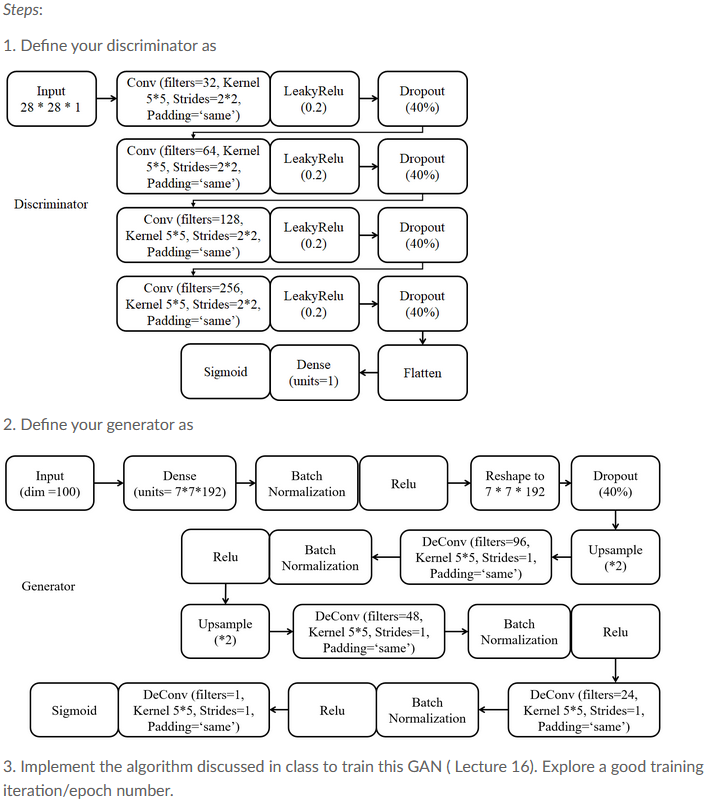
\includegraphics[width=4in]{csci-8110/hw-4/images/8110_hw4_diagram.png}
    \caption{The schema of the discriminator (top) and generator (bottom). From assignment description.}
    \label{fig:diagram}
\end{figure}

With the models defined, a full generative adversarial network (GAN) could be constructed using the algorithm discussed in class:

\begin{figure}[H]
    \centering
    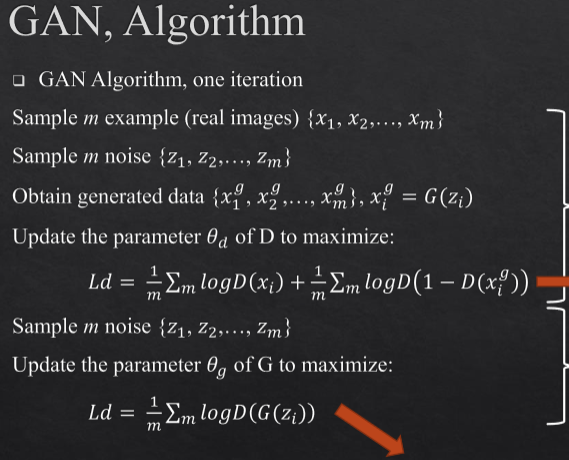
\includegraphics[width=4in]{csci-8110/hw-4/images/8110_hw4_algorithm.png}
    \caption{Pseudocode GAN algorithm}
    \label{fig:algo}
\end{figure}

\subsection{Implementation} \label{impl}
\par The first step toward this assignment involved implementing the two models defined in the assignment description. 
The code for these, being more or less a completely by-the-numbers implementation of explicitly defined layers, was trivial to write and is included in the \nameref{codelist} section.
Combining the models together was a straightforward process as well, adding both independent models to a new "parent" model:

\begin{lstlisting}[language=Python]
print('defining discriminator')
discriminator = discriminator_impl()
discriminator.trainable = False
print('defining generator')
generator = generator_impl()
print('defining gan')
gan = Sequential()
gan.add(generator)
gan.add(discriminator)
opt = Adam(lr=0.0002, beta_1=0.5)
gan.compile(loss='binary_crossentropy', optimizer=opt)
\end{lstlisting}

\par Note that the discriminator model was set such that \lstinline{trainable = False}.

\par Of more consequence was the process of supplying data to the complete model, training it, and plotting the results. 
For purposes of this assignment, 600 epochs were run, each with a fairly standard batch size of 256.
In each iteration, images need to be randomly selected from the provided MNIST data.
Keras makes loading that data fairly straightforward with the \lstinline{load_data()} function:

\begin{lstlisting}[language=Python]
def load_images():
	# load mnist dataset
	(train_data, _), (_, _) = load_data()
	X = expand_dims(train_data, axis=-1)
	X = X.astype('float32')
	X = X / 255.0
	return X
\end{lstlisting}

\par On top of random selection, the data needed to be marked as "real data" with an array of ones:

\begin{lstlisting}[language=Python]
# select real samples
def get_real_data(dataset, num_samples):
	random_selector = randint(0, dataset.shape[0], num_samples)
	x = dataset[random_selector]
	# label as real
	y = ones((num_samples, 1))
	return x, y
\end{lstlisting}

\par Next, "fake" images were generated and marked with zeros using the generator model defined in the assignment guidelines:

\begin{lstlisting}[language=Python]
# use the generator to generate fresh images
def get_fake_data(generator, dim_value, num_samples):
	x_input = randn(dim_value * num_samples)
	x_input = x_input.reshape(num_samples, dim_value)
	# based on random input, generate images from noise
	x = generator.predict(x_input)
	# label as fake samples
	y = zeros((num_samples, 1))
	return x, y
\end{lstlisting}

\par In each epoch's batch, half of the data was real, and half was fake, and the discriminator was trained on the supplied data:

\begin{lstlisting}[language=Python]
# pick random images from MNIST dataset
x_real, y_real = get_real_data(dataset, 128)
# generate fake images
x_fake, y_fake = get_fake_data(generator, dim_value, 128)
# combine two sets of images into one set of size 256
x, y = vstack((x_real, x_fake)), vstack((y_real, y_fake))
discriminator_loss, _ = discriminator.train_on_batch(x, y)
\end{lstlisting}

\par Finally, one more set of random points was generated and marked as "real" for input to the full GAN model:

\begin{lstlisting}[language=Python]
# set up random points in latent space for generator input
x_input = randn(dim_value * batch_size)
x_input = x_input.reshape(batch_size, dim_value)
# label samples as real, for testing
y_input = ones((batch_size, 1))
# get gan loss
gan_loss = gan.train_on_batch(x_input, y_input)
\end{lstlisting}

\par With the model trainable, training can begin, and outputs can be measured.

\subsection{Model Observations} \label{model_obvs}
\par Using the plots generated in the code, it's possible to draw some interesting conclusions about the GAN model implemented for this assignment.
The output of the first epoch is shown in the epoch below:

\begin{figure}[H]
    \centering
    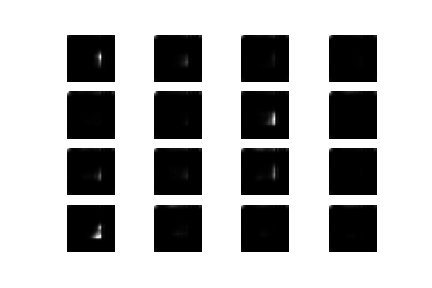
\includegraphics[width=4in]{csci-8110/hw-4/images/generated_plot_e001.png}
    \caption{Generated images after first epoch}
    \label{fig:ep1}
\end{figure}

\par At this point, it's fairly clear that the output of the generator still contains a good deal of noise.
By the tenth epoch, the noise from the output is already visibly reduced:

\begin{figure}[H]
    \centering
    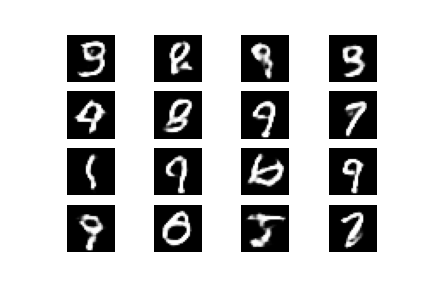
\includegraphics[width=4in]{csci-8110/hw-4/images/generated_plot_e010.png}
    \caption{Generated images after tenth epoch}
    \label{fig:ep10}
\end{figure}

\par By the hundredth epoch things have improved considerably:

\begin{figure}[H]
    \centering
    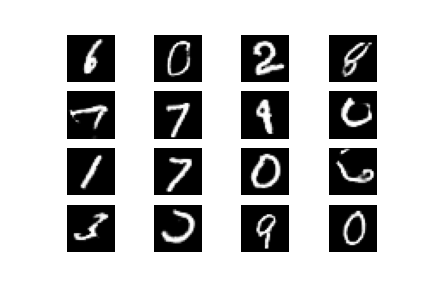
\includegraphics[width=4in]{csci-8110/hw-4/images/generated_plot_e100.png}
    \caption{Generated images after 100th epoch}
    \label{fig:ep100}
\end{figure}

\par By now, interesting behavior starts to become visible--subsequent epochs don't seem to meaningfully improve the model outputs--between the 100th epoch and the 600th epoch, things don't seem to dramatically improve:

\begin{figure}[H]
    \centering
    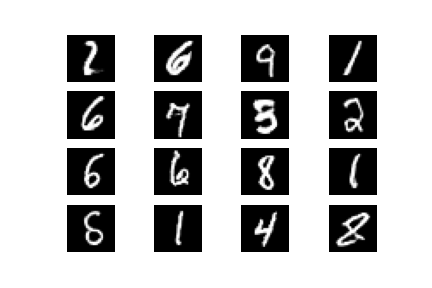
\includegraphics[width=4in]{csci-8110/hw-4/images/generated_plot_e600.png}
    \caption{Generated images after 600th epoch}
    \label{fig:ep600}
\end{figure}

\par This observation is further supported by an analysis of the loss values of the discriminator and GAN models from every iteration of the training algorithm, plotted in Microsoft Excel:

\begin{figure}[H]
    \centering
    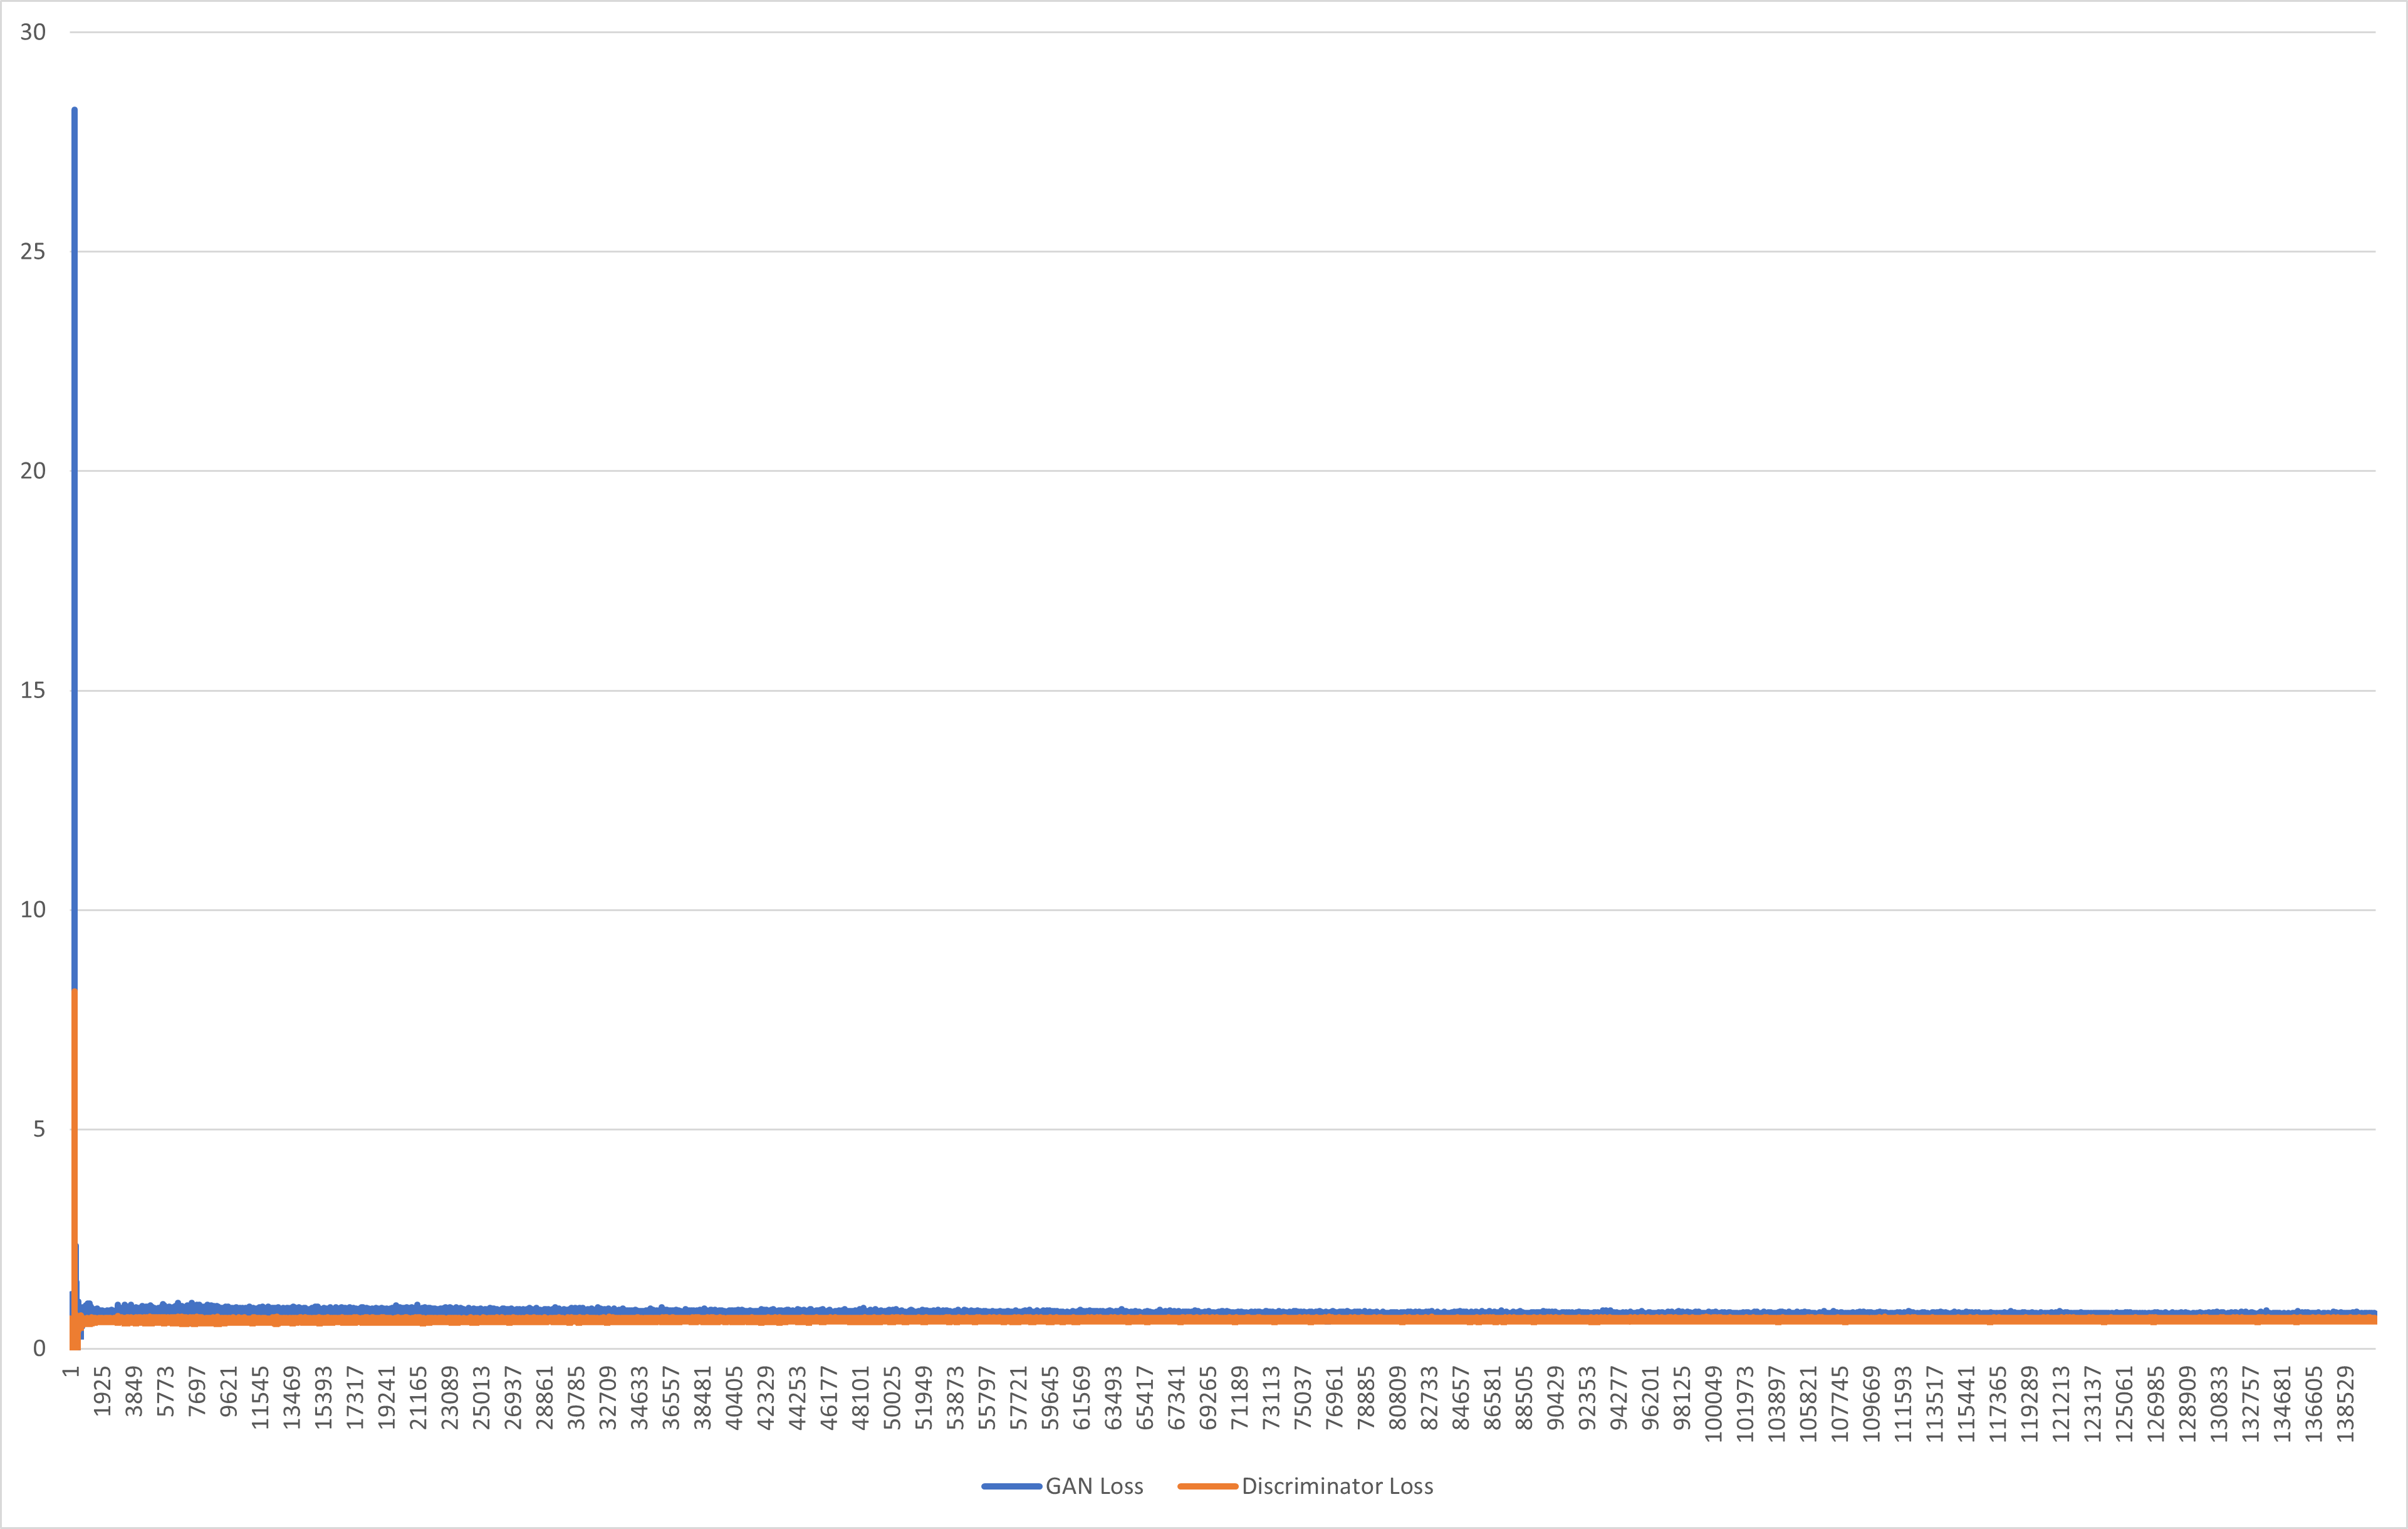
\includegraphics[width=6in]{csci-8110/hw-4/images/8110_hw4_loss.png}
    \caption{Loss Graph}
    \label{fig:loss_graph}
\end{figure}

\par As can be seen in the graph above, loss values fluctuate wildly across iterations to start but stabilize substantially to values between 0.600 and 0.700.
This stabilization of the GAN model is fairly well documented in academic papers and indicates that more epochs with the same model do not necessarily increase the quality of outputs.
It demonstrates the value in supervised training--in situations like this one it's entirely possible to do "too much" work--wasting resources on training iterations that do not improve the quality of outputs.
A "zoomed in" graph showing this stabilization across the first ten epochs is included in the \nameref{graph_app} appendix.
A complete listing of model outputs is included in the \nameref{modelouts} appendix.

\section{Conclusions}
\par This assignment over GANs entailed some of the most interesting work of the semester to date.
It also brings together the concepts of defining, training, and validating convolutional neural networks used throughout the semester in the 8110 course material in a single comprehensive project.
Having an opportunity to build, train, and display results from a neural network that generates its own content is a great start down the path toward understanding how machine learning applications can be used as tools to generate and evaluate content, when supervised correctly.
The takeaways from this assignment--and the course as a whole--provide tremendous value as a basis upon which more knowledge in machine learning can be developed.
% \bibliographystyle{unsrt}
% \bibliography{references}

\begin{appendices}
\newpage
\section{Complete Code Listing} \label{codelist}
\lstinputlisting[language=Python]{8110_hw4.py}
\newpage
\section{Stabilization Graph} \label{graph_app}
\begin{figure}[H]
    \centering
    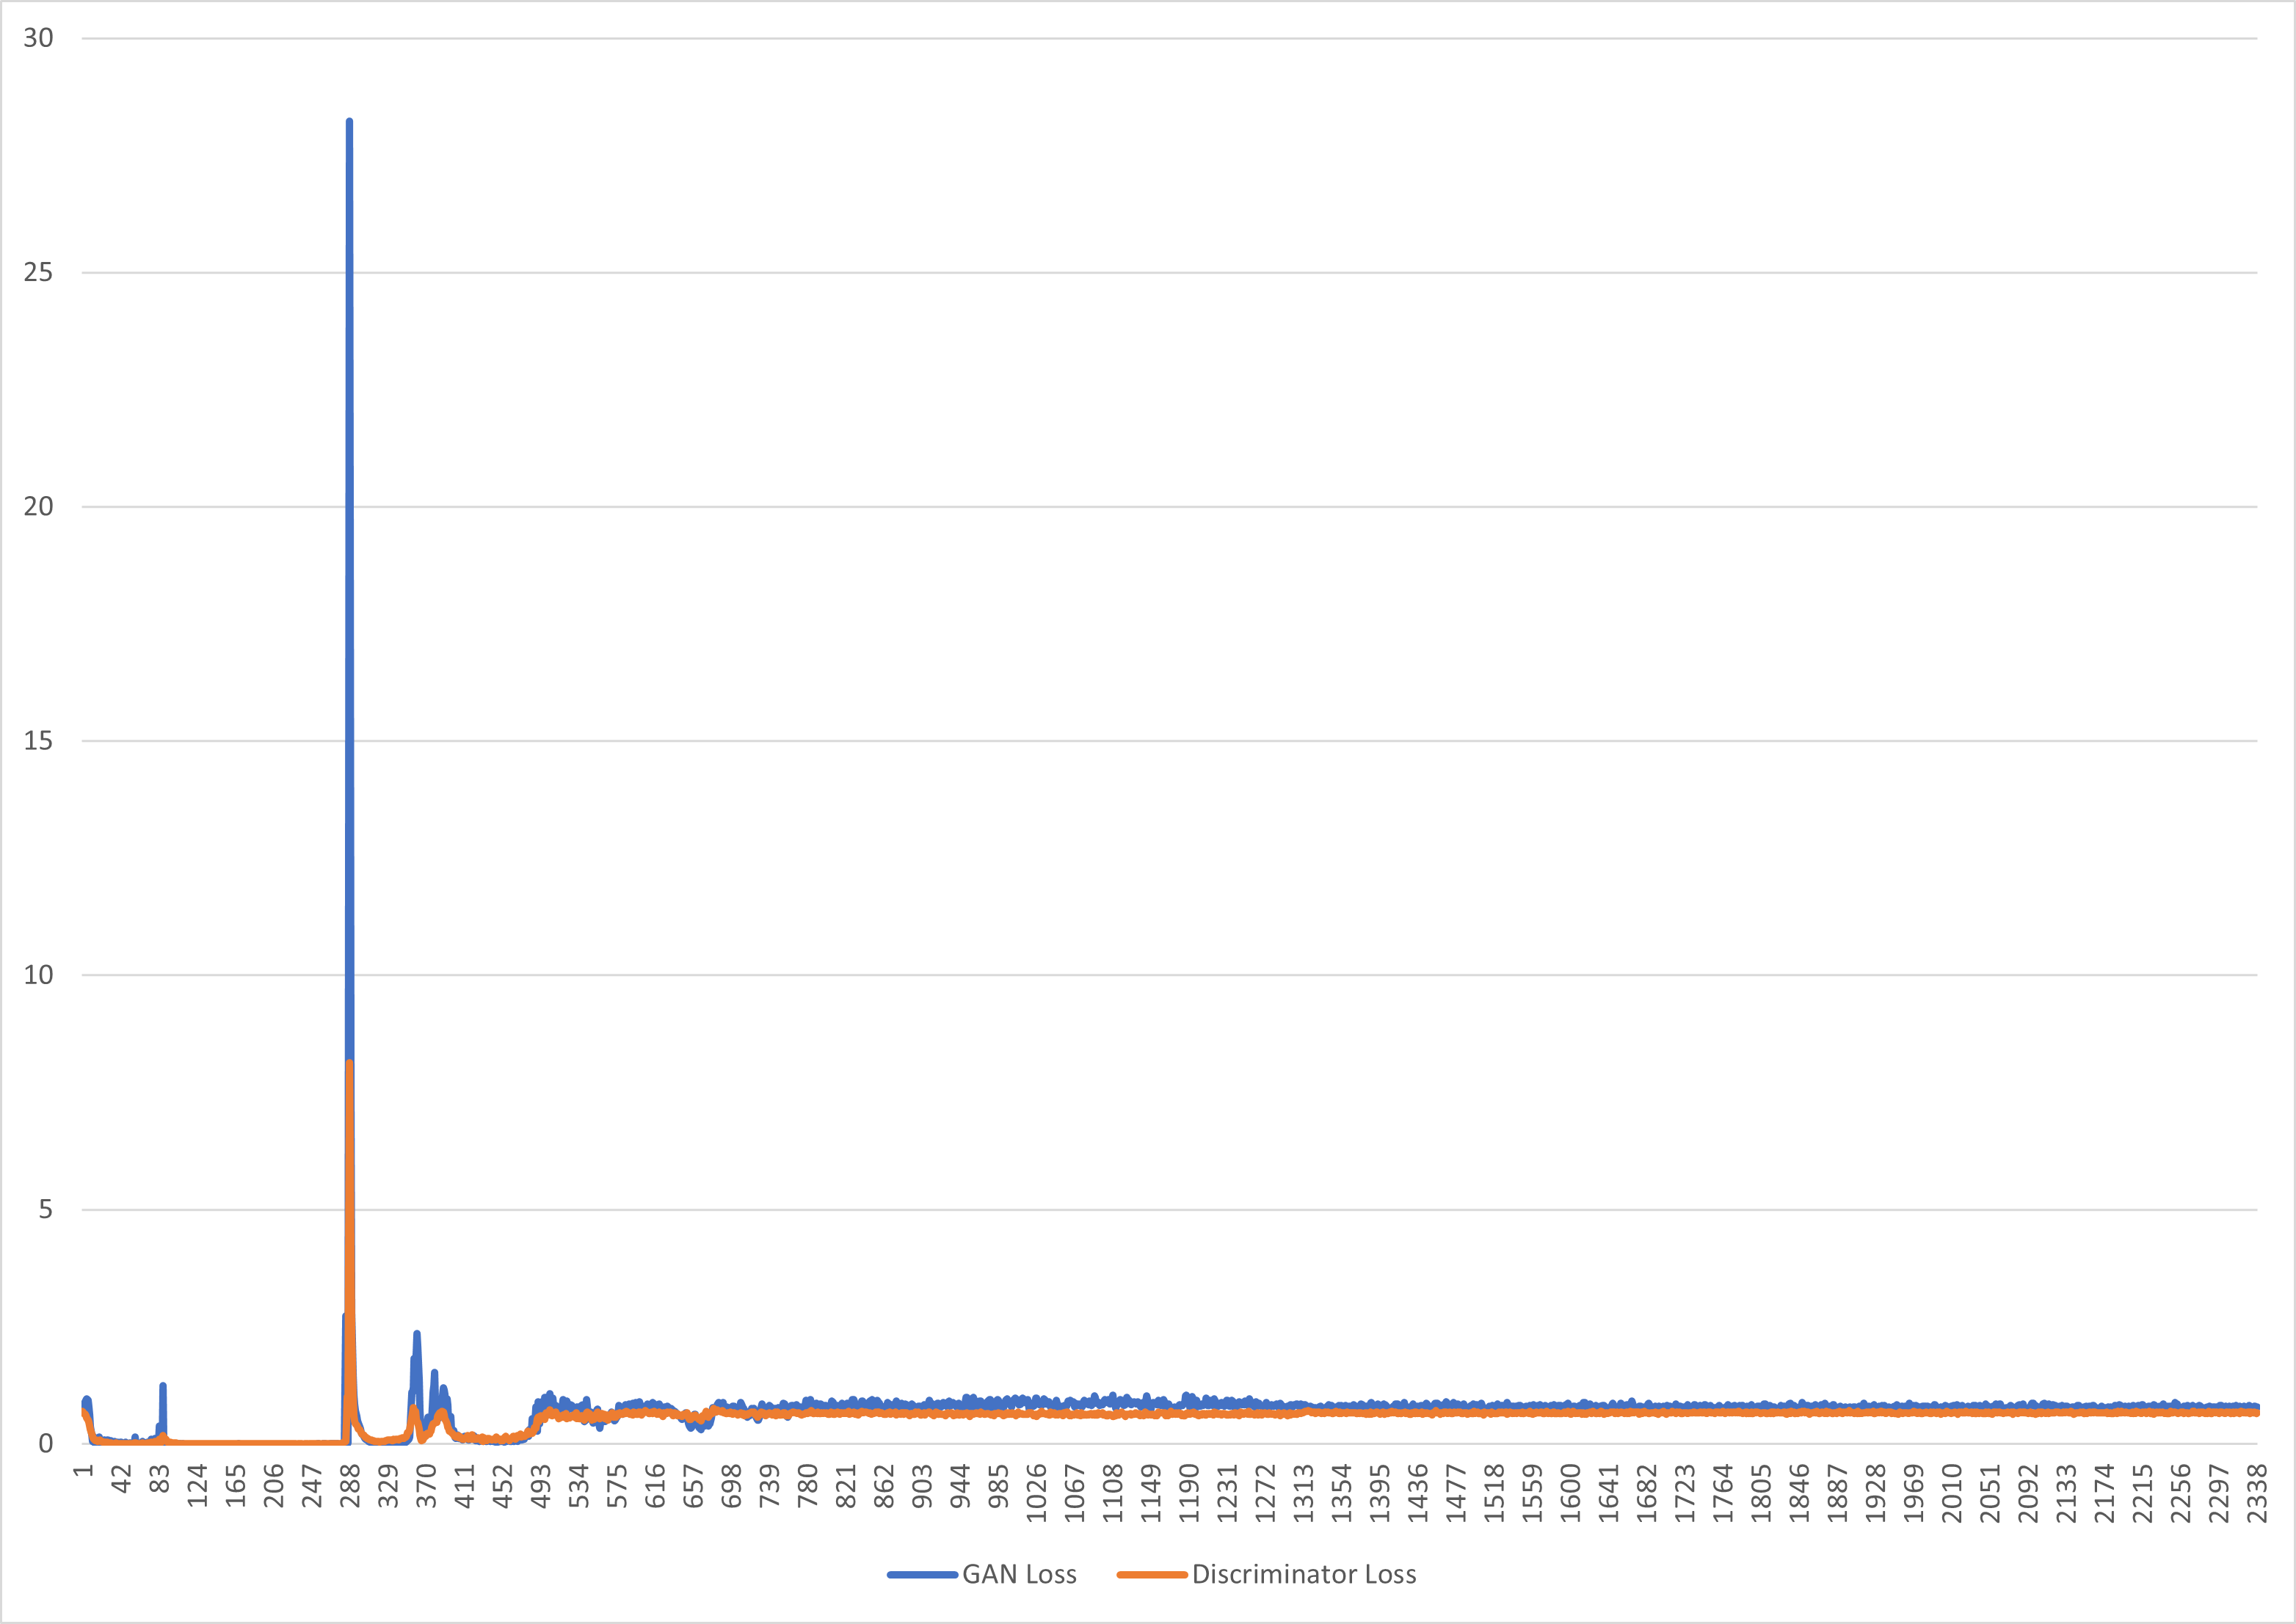
\includegraphics[width=6in]{csci-8110/hw-4/images/8110_hw4_loss_first_10.png}
    \caption{Loss Graph: First 10 Epochs}
    \label{fig:loss_graph_10}
\end{figure}

\newpage
\section{Model Output Listing} \label{modelouts}

\begin{figure}[H]
\centering
\begin{subfigure}{.5\textwidth}
  \centering
  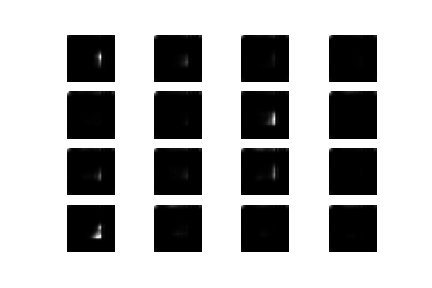
\includegraphics[width=3in]{csci-8110/hw-4/images/generated_plot_e001.png}
  \label{fig:ep1_2}
\end{subfigure}%
\begin{subfigure}{.5\textwidth}
  \centering
  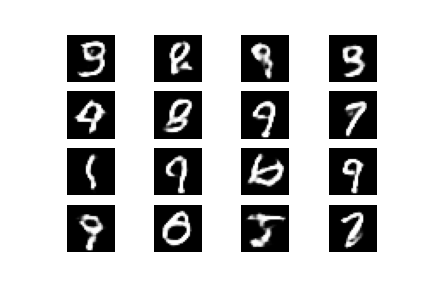
\includegraphics[width=3in]{csci-8110/hw-4/images/generated_plot_e010.png}
  \label{fig:ep100}
\end{subfigure}
\caption{Outputs after first epoch (left) and tenth epoch (right)}
\label{fig:ep1-10}
\end{figure}

\begin{figure}[H]
\centering
\begin{subfigure}{.5\textwidth}
  \centering
  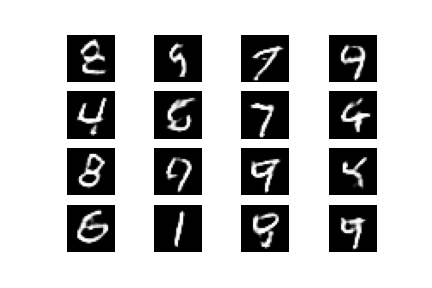
\includegraphics[width=3in]{csci-8110/hw-4/images/generated_plot_e020.png}
  \label{fig:ep20}
\end{subfigure}%
\begin{subfigure}{.5\textwidth}
  \centering
  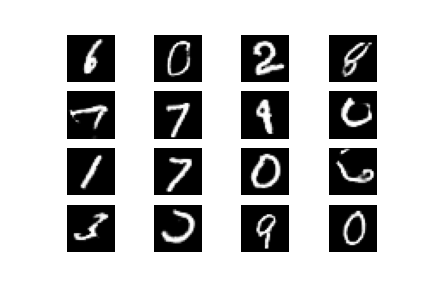
\includegraphics[width=3in]{csci-8110/hw-4/images/generated_plot_e100.png}
  \label{fig:ep100_2}
\end{subfigure}
\caption{Outputs after 20th epoch (left) and 100th epoch (right)}
\label{fig:ep20-100}
\end{figure}

\begin{figure}[H]
\centering
\begin{subfigure}{.5\textwidth}
  \centering
  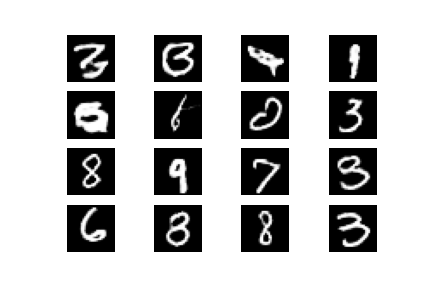
\includegraphics[width=3in]{csci-8110/hw-4/images/generated_plot_e150.png}
  \label{fig:ep150}
\end{subfigure}%
\begin{subfigure}{.5\textwidth}
  \centering
  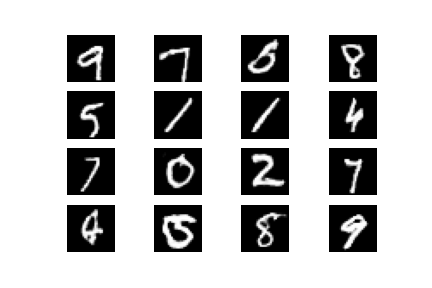
\includegraphics[width=3in]{csci-8110/hw-4/images/generated_plot_e200.png}
  \label{fig:ep200}
\end{subfigure}
\caption{Outputs after 150th epoch (left) and 200th epoch (right)}
\label{fig:ep20-100}
\end{figure}

\begin{figure}[H]
\centering
\begin{subfigure}{.5\textwidth}
  \centering
  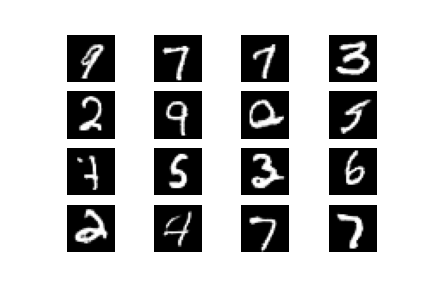
\includegraphics[width=3in]{csci-8110/hw-4/images/generated_plot_e250.png}
  \label{fig:ep250}
\end{subfigure}%
\begin{subfigure}{.5\textwidth}
  \centering
  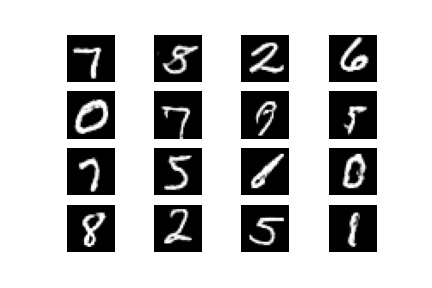
\includegraphics[width=3in]{csci-8110/hw-4/images/generated_plot_e300.png}
  \label{fig:ep300}
\end{subfigure}
\caption{Outputs after 250th epoch (left) and 300th epoch (right)}
\label{fig:ep20-100}
\end{figure}

\begin{figure}[H]
\centering
\begin{subfigure}{.5\textwidth}
  \centering
  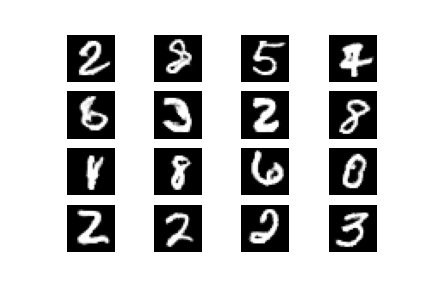
\includegraphics[width=3in]{csci-8110/hw-4/images/generated_plot_e350.png}
  \label{fig:ep20}
\end{subfigure}%
\begin{subfigure}{.5\textwidth}
  \centering
  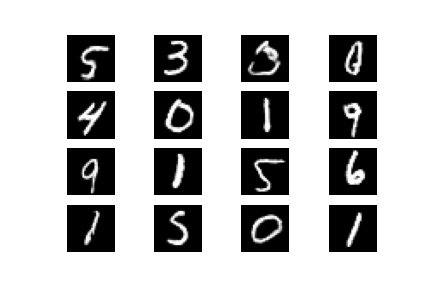
\includegraphics[width=3in]{csci-8110/hw-4/images/generated_plot_e400.png}
  \label{fig:ep100_2}
\end{subfigure}
\caption{Outputs after 350th epoch (left) and 400th epoch (right)}
\label{fig:ep20-100}
\end{figure}

\begin{figure}[H]
\centering
\begin{subfigure}{.5\textwidth}
  \centering
  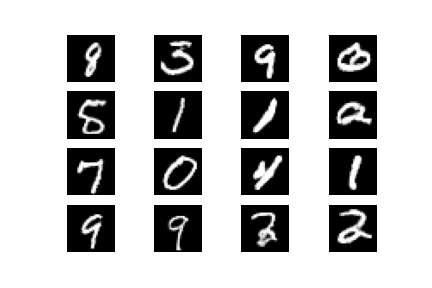
\includegraphics[width=3in]{csci-8110/hw-4/images/generated_plot_e450.png}
  \label{fig:ep20}
\end{subfigure}%
\begin{subfigure}{.5\textwidth}
  \centering
  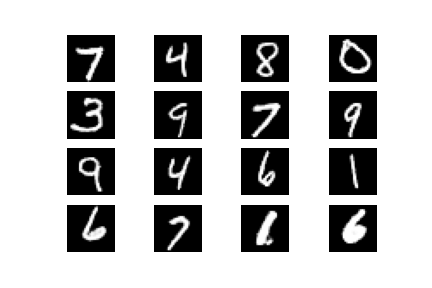
\includegraphics[width=3in]{csci-8110/hw-4/images/generated_plot_e500.png}
  \label{fig:ep100_2}
\end{subfigure}
\caption{Outputs after 450th epoch (left) and 500th epoch (right)}
\label{fig:ep20-100}
\end{figure}

\begin{figure}[H]
\centering
\begin{subfigure}{.5\textwidth}
  \centering
  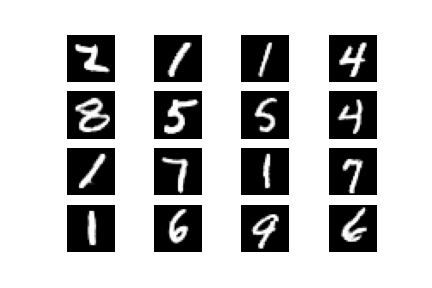
\includegraphics[width=3in]{csci-8110/hw-4/images/generated_plot_e550.png}
  \label{fig:ep20}
\end{subfigure}%
\begin{subfigure}{.5\textwidth}
  \centering
  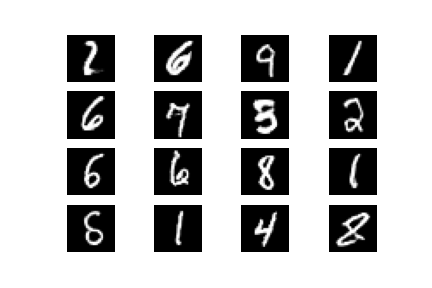
\includegraphics[width=3in]{csci-8110/hw-4/images/generated_plot_e600.png}
  \label{fig:ep100_2}
\end{subfigure}
\caption{Outputs after 550th epoch (left) and 600th epoch (right)}
\label{fig:ep20-100}
\end{figure}

\end{appendices}

\end{document}